\documentclass{book}

\usepackage{hyperref}
\usepackage{graphicx}
\usepackage[letterpaper, margin=1in]{geometry}
\usepackage{amsmath}
\usepackage{amsfonts}
\newtheorem{definition}{Definition}


\graphicspath{{./fig/}}

\title{Lie Groups in Robotics}
\author{James Goppert}
\date{January 22, 2023}

\begin{document}

\maketitle
\tableofcontents

\chapter{Introduction}

This book is aimed at introducing graduate and undergraduate students
in engineering to the applications of Lie groups theory that are 
relevant to engineering. Instead of focusing on the abstract 
mathematics initially, it will build intuition by traversing the most
fundamental Lie Groups in robotics.

\section{What is a Lie Group}

\begin{definition}
A \href{https://en.wikipedia.org/wiki/Group_(mathematics)}{Group} is a set G
and an associated operator $\cdot$ that is:
\begin{itemize}
    \item \textbf{C}losed: if $a \in G$ and $b \in G$, then $a \cdot b \in G$
    \item \textbf{A}ssociative: $(a \cdot b) \cdot c = a (\cdot b \cdot c)$
    \item \textbf{I}nverse: $a^{1}\cdot a = e$
    \item \textbf{N}eutral: $a \cdot e = e$
\end{itemize}
\end{definition}

\begin{definition}
    A \href{https://en.wikipedia.org/wiki/Lie_group}{Lie Group} is a group that
    is also a differentiable manifold.
    \end{definition}

A \href{https://en.wikipedia.org/wiki/Differentiable_manifold}{differentiable manifold}
is a topological space resemlbling Euclidean space near each point
and locally similar enough to a vector space to apply calculus. Originally Lie Groups were called infinitesmal groups by the creator
\href{https://en.wikipedia.org/wiki/Sophus_Lie}{Sophus Lie} (pronounced Lee).
The can be thought of as groups of continuous transformations.

\begin{figure}[htp]
    \centering
    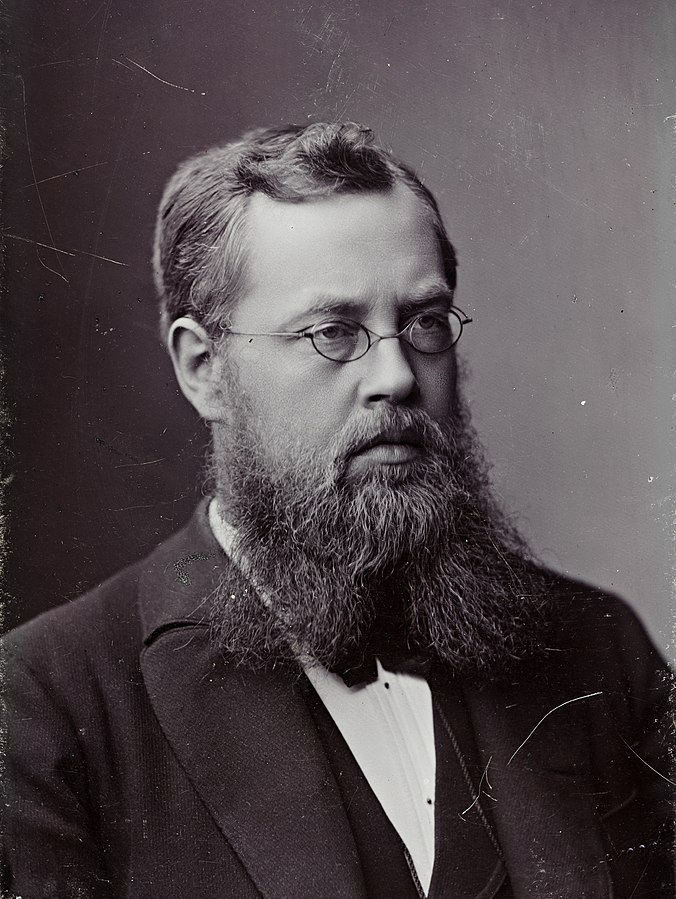
\includegraphics[width=100px]{sophus_lie}
    \caption{Sophus Lie}
\end{figure}

\section{Applications of Lie Groups}

\subsection*{Covered in this Course}
\begin{itemize}
    \item Estimation
        \begin{itemize}
            \item IEKF : Invariant Extended Kalman Filter
            \item Simultaneous Localization and Mapping
        \end{itemize}
    \item Control of Rigid Bodies
        \begin{itemize}
            \item Reachable set calculations
            \item Geometric control
        \end{itemize}
    \item Computer Vision
    \begin{itemize}
        \item Perspective Transforms
        \item Homogenous Coordinates
    \end{itemize}
\end{itemize}


\subsection*{Others Topics not Covered}
\begin{itemize}
    \item Quantum mechanics
\end{itemize}


\section*{Excercises}

\subsection*{Questions about Groups}

\begin{itemize}
    \item Is the set of all Integers $\mathbb{Z}$ with the addition operator $+$ a group?
    \item Is the set of all Integers $\mathbb{Z}$ with the multiplication operator $*$ a group?
    \item Is the set of all $n\times n$ matrices with the matrix multiplication oerator a group?
\end{itemize}

\subsection*{Questions about Lie Groups}
\begin{itemize}
    \item Is the set of all Integers $\mathbb{Z}$ with the addition operator $+$ a Lie group?
    \item Is the set of all Real numbers $\mathbb{R}$ with the addition operator $+$ a Lie group?
\end{itemize}


\chapter{The $SO(2)$ Lie Group}
%
\section{Group Representation}
%
$SO(2)$ can be represented by any matrix of the from:
%
$$G(\theta) = \begin{bmatrix}
\cos{\theta} & -\sin{\theta} \\
\sin{\theta} & \cos{\theta}
\end{bmatrix}$$
with the Group operator of matrix multiplication ($\cdot$), where $\theta \in \mathbb{R}$.

To show that $SO(2)$ is a Lie Group, we much show that it is closed, associative, has inverse, and a neutral element and is a differentiable manifold

\subsection*{Closed}
%
Since $G(\theta_1) \cdot G(\theta_2) = G(\theta_1 + \theta_2)$, $SO(2)$ is \textbf{closed} under matrix multiplication.

\subsection*{Associative}
%
$SO(2)$ as a Matrix Lie Group, can inheret associativity from matrix multiplication:
%
$$(A \cdot B) \cdot C = A \cdot (B \cdot C)$$

\subsection*{Inverse}
%
$SO(2)$ as a Matrix Lie Group, can inheret the inverse from matrix multiplication, since any element of $SO(2)$ has a non-zero determinant (1) and is invertible.
%
$$\det{G} = \cos^2{\theta} + \sin^2{\theta} = 1$$
%
Because the columns of $G(\theta)$ are orthonomal, the inverse is given by the matrix transpose.
%
$$G^{-1}(\theta) = G^T(\theta)$$

\subsection*{Neutal}
%
$SO(2)$ as a Matrix Lie Group, can inheret the neutral element from matrix multiplication, $I$.
%
$$A\cdot I = A$$

\subsection*{Differential Manifold}
Is is clear that the group $SO(2)$ is continuous as it inherits this from $\mathbb{R}$.
$G(\theta)$, $\theta \in \mathbb{R}$.
We will see in the Lie Algebra that the group is locally similar to 1 dimensional Euclidean space
and we can perform calculus.


\section{Lie Algebra}
%
For matrix Lie groups, we can always find an element of the Lie Algebra, $\Omega$ via:
%
$$\dot{G} = G\Omega$$
%
$$\Omega = G^{-1}\dot{G}$$
%
The so2 Lie algebra can be represented by all 2x2 skew symmetric matrices of the form:
%
$$\Omega = \begin{bmatrix}
0 & - \omega\\
\omega & 0
\end{bmatrix}$$
%
It is convenient to define a wedge operator such that:

\begin{definition}[The Wedge Operator]
$$\mathbb{R} \mapsto so(2)$$
$$\omega^{\wedge} = \begin{bmatrix}
    0 & - \omega\\
    \omega & 0
    \end{bmatrix}$$
\end{definition}
%
It is also convient to define a vee operator, the inverse of the wedge operator such that:
%
\begin{definition}[The Vee Operator]
$$so(2) \mapsto \mathbb{R}$$
$$\begin{bmatrix}
0 & - \omega\\
\omega & 0
\end{bmatrix}^{\vee} = \omega$$
\end{definition}

\end{document}